\subsection{En pratique}

\begin{frame}{Implémentation (\textsc{Python 3})}
    \begin{alertblock}{État de l'implémentation}
    \begin{itemize}
    \item Création des clefs: \checked
    \item Chiffrement : \checked
    \item Déchiffrement : \checked
    \item Somme : \checked
    \item Produit : \checked
    \item Bootstrap : Échec
\end{itemize}
    \end{alertblock}{}
    
    \begin{alertblock}{Paramètres de base}
    Ceux proposés par l'article
    \end{alertblock}{}
\end{frame}


\begin{frame}
\frametitle{Constatation des performances}
\framesubtitle{Génération des clefs}
\begin{center}
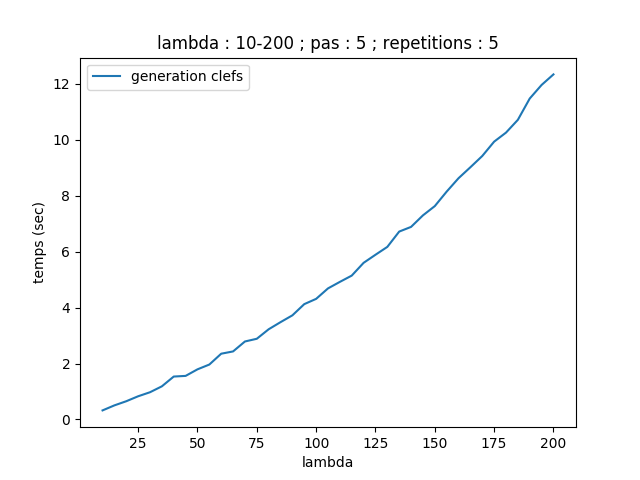
\includegraphics[scale=0.46]{images/generation_clefs.png} 
\end{center}
\end{frame}

\begin{frame}
\frametitle{Constatation des performances}
\framesubtitle{Génération des chiffrés}
\begin{center}
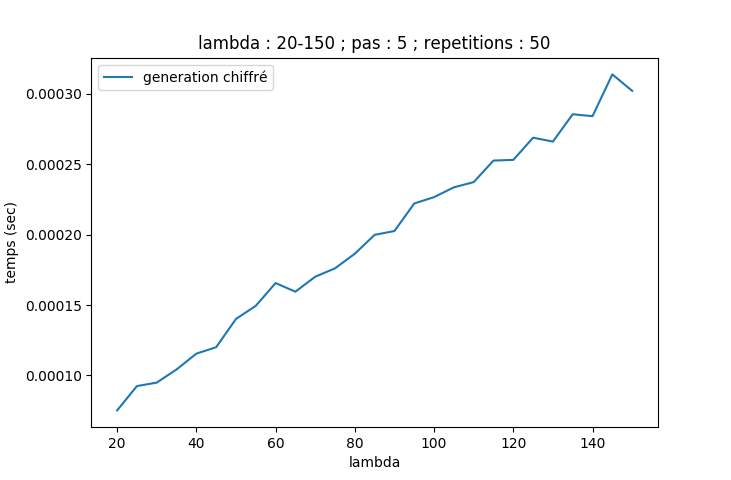
\includegraphics[scale=0.46]{images/generation_chiffre2.png} 
\end{center}
\end{frame}

\begin{frame}
\frametitle{Constatation des performances}
\framesubtitle{Somme}
\begin{center}
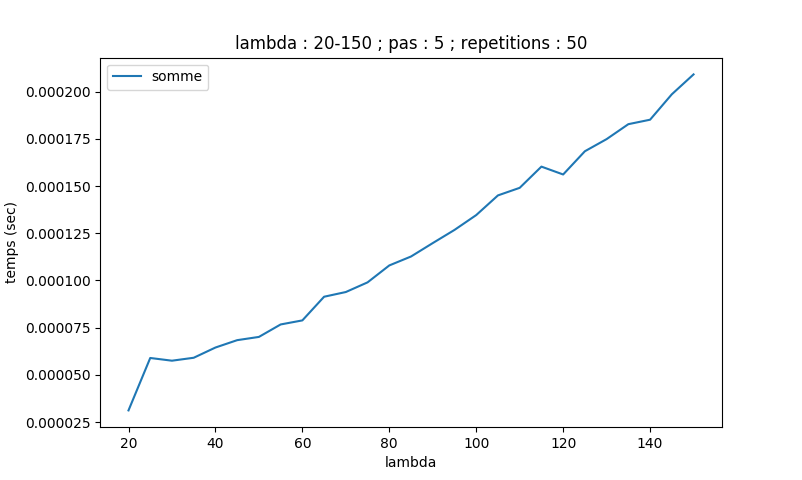
\includegraphics[scale=0.46]{images/somme.png} 
\end{center}
\end{frame}

\begin{frame}
\frametitle{Constatation des performances}
\framesubtitle{Produit}
\begin{center}
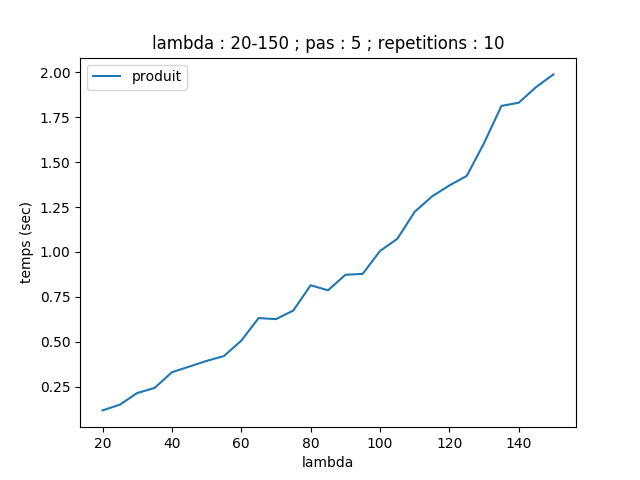
\includegraphics[scale=0.46]{images/produit.png} 
\end{center}
\end{frame}

\begin{frame}{Constatation des performances}
\framesubtitle{Nombre d'opérations}
    \begin{alertblock}{Nombre d'opérations}
    \textbf{Dérisoire} $\to$ 4 ou 5 multiplications bit à bit avant erreur
    \end{alertblock}{}
\end{frame}{}
% d'ou ENJEU


\begin{frame}
\frametitle{Le bootstrap}
\begin{alertblock}{Échec}
En cause :
\begin{itemize}
    \item \textbf{Schéma trop théorique} et peu adapté à une implémentation
    \item \textbf{Évaluation homomorphique} des fonctions de chiffrement et déchiffrement \textbf{trop gourmande en calculs} et donc incompatible avec des paramètres pertinents pour un ordinateur
\end{itemize}{}
    \end{alertblock}
\end{frame}